\section{Optimierung}
Nachdem wir nun wissen wie bei der Evaluierung aus der
Mozart/Oz-Darstellung der abstrakten Syntax die Mozart/Oz Constraints
generiert werden, widmen wir uns jetzt der Optimierung, die noch vor
der Evaluierung stattfindet.

Wir wissen jetzt, dass jeder Quantor in der PrincipleWriter User
Language in eine {\tt for}-Schleife umgesetzt wird, die \"uber die
Elemente des Typs der Variable iteriert. Die Ausf\"uhrungzeit steigt
damit linear zur M\"achtigkeit dieses Typs.  Mit jeder Schachtelung
von Quantoren steigt die Anzahl von letztendlich gestarteten
Propagierern, was sich leicht negativ auf die Laufzeit auswirken kann.

Experten im Schreiben von Prinzipien als Mozart/Oz-Constraints
k\"onnen die verschiedenen Knotenmengen ausnutzen, die bei der
Modellierung des Multigraphen gebildet werden. Sie k\"onnen damit die
Anzahl von Quantoren, und deren Schachtelung reduzieren. Aus einigen
dieser Techniken konnte ich Muster erkennen, die regelm\"a{\ss}ig
vorkommen.

Der Optimierer automatisiert einige dieser Techniken.  Er durchwandert
den durch die Typinferenz vollst\"andig getypten Parsebaum und
versucht durch Pattern-Matching Muster zu erkennen, f\"ur die
Optimierungen bekannt sind. Wird ein Muster gefunden, ersetzt der
Optimierer den Teilbaum, der das Muster im Parsebaum repr\"asentiert,
durch einen neuen Teilbaum, der die Optimierung repr\"asentiert. In
der Evaluation wird dann die entsprechende optimierte Funktion aus der
PW-Bibliothek eingesetzt, die das Problem so l\"ost, wie Experten es
tun w\"urden.

Der Optimierer findet derzeit nicht alle diese Muster, die er
optimieren kann, da manche Muster verschiedene \"aquivalente
Darstellungen in den logischen Formeln haben, z.B.\ gilt
$\forall~x:F~\equiv~\neg~\exists~x:~\neg~F$. Um dieses Problem zu
beheben, m\"ussten die Formeln vor dem Patternmatching in eine Art
Normalform \"uberf\"uhrt werden, was bisher noch nicht gemacht wird,
aber einen interessanten Ansatz f\"ur weitere Forschungen bietet, die
generierten Prinzipien noch besser zu optimieren.

Wie die Verwendung der Knotenmengen die Anzahl der Quantifizierungen
und die verschachtelungstiefe der Quantifizierungen verringern kann,
schauen wir uns an Beispielen an.

\subsection{ZeroOrOneMother}

Die {\it ZeorOrOneMother}-Optimierung kann z.B.\ einen Constraint des
Baumprinzips erheblich verbessern. Zur Erinnerung, der Constraint wird
in First-Order Logik so beschrieben:
$$\forall v:(\neg \exists v' : v' \rightarrow_d v) \vee
(\exists^1 v' \rightarrow_d v)$$ 
Bei der unoptimierten Evaluation w\"urde ein Mozart/Oz-Constraint
generiert, der verschachtelte Quantoren enth\"alt, die
Verschachtelungstiefe w\"are 1.

Die Idee der Optimierung folgt direkt aus den beiden Komponenten der
Disjunktion. Die linke Seite der Disjunktion pr\"uft, ob der Knoten
$v$ aus der \"au{\ss}eren Quantifizierung keine Mutter hat. Da bei der
Modellierung des Multigraphen f\"ur jeden Knoten eine Menge {\tt
  mothers} gebildet wird, die alle M\"utter des Knotens enth\"alt,
muss nicht f\"ur jeden Knoten gepr\"uft werden, ob er eine Mutter von
$v$ ist. Es reicht zu \"uberpr\"ufen, ob die Muttermenge von $v$ leer
ist. Die rechte Seite pr\"uft, ob der Knoten $v$ genau eine Mutter
hat. Anstatt daf\"ur \"uber alle Knoten zu iterieren, reicht es zu
pr\"ufen, ob die Muttermenge von $v$ genau ein Element enh\"alt.

Ob die Muttermenge leer ist oder genau ein Element enth\"alt kann
\"uber die Kardinalit\"at der Menge festgestellt werden. Der erste
Optimierungsschritt sieht dann so aus:
$$\forall v: \underbrace{(\neg \exists v' : v' \rightarrow_d v)
}_{|\mathit{mothers(v)}| = 0}\vee
\underbrace{(\exists^1 v' \rightarrow_d v)}_{|\mathit{mothers(v)}| = 1}$$

Der n\"achste Optimierungsschritt eliminiert die Disjunktion, indem
nur noch gepr\"uft wird, ob die Kardinalit\"at der Muttermenge $\leq$
1 ist. Die vollst\"andig optimierte Formel sieht jetzt so aus:
$$\forall v: |mothers(v)| \leq 1$$
Sie enth\"alt nur noch eine Quantifizierung und es m\"ussen weniger
Propagierer gestartet werden als im ersten Optimierungsschritt.

Der Optimierer arbeitet durch Patternmatching auf der Mozart/Oz
Darstellung der abstrakten Syntax. F\"ur die Beispiel-Optimierung
sucht er ein Pattern der Form:
\begin{verbatim}
disj(neg(exists(X _ edge(Y Z D)))
     existsone(X _ edge(Y Z D)))
\end{verbatim}
mit $Z \neq Y$. Ein gefundener Unterbaum dieser Form wird durch einen
neuen Baum der Form:
\begin{verbatim}
zeroOrOneDaughters(Z D)
\end{verbatim}
ersetzt, und damit auch die abstrakte Syntax erweitert.  Bei der
Evaluierung wird die entsprechende optimierte Funktion aus der {\tt
  PW}-Bibliothek benutzt. F\"ur die Beispieloptimierung sieht sie so
aus:
\begin{center}
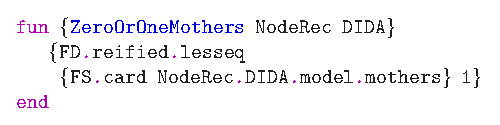
\includegraphics[scale=1.0]{eps/opti}
\end{center}

\subsection{Disjunktheit von Unterb\"aumen mit unterschiedlichem Label}
Den bei der Evaluierung vorgestellten Constraint wollen wir hier
nochmal aufgreifen. Der Constraint verlangt, dass die Unterb\"aume
eines Knotens mit unterschiedlichem Label disjunkt sein m\"ussen.  Aus
der Formel des Constraints:
$$\forall v: \forall v' : \forall l: \forall l': v
 \overset{l}{\rightarrow}_d \rightarrow_d^* v' \wedge v
 \overset{l'}{\rightarrow}_d \rightarrow_d^* v' \Rightarrow l=l'
$$
ist zu erkennen, dass zweimal verschachtelt quantifiziert wird. Einmal
 \"uber die Knoten und einmal \"uber die Kantenbeschriftungen.

Wenn wir uns \"uberlegen, was die geforderte Disjunktheit bedeutet,
wird die Optimierung leicht klar. Der Constraint verlangt, dass es in
jedem Knoten keine zwei ausgehenden Kanten mit der gleichen
Beschriftung geben darf. Das bedeutet, dass es keine verschiedenen
Pfade von einem Knoten $v$ zu einem Knoten $v'$ aus der Menge
$\mathit{down}$ der Knoten unterhalb von $v$ geben darf, deren erste
Kante das gleiche Label hat.

Die Menge $\mathit{downL}$ enth\"alt Paare aus einem Label und einer
Untermenge der Knoten aus $\mathit{down}$. F\"ur jede ausgehende Kante
$l$ des Knotens $v$ wird solch ein Paar gebildet. Die Untermengen
enthalten die Knoten, die von $v$ \"uber die Kante $l$ erreicht werden
k\"onnen. Wenn die Unterb\"aume mit unterschiedlichem Label disjunkt
sind, bilden die Untermengen aus $\mathit{downL}$ eine Partition von
$\mathit{down}$. Die Optimierung sieht jetzt so aus, dass nur noch
f\"ur jeden Knoten gepr\"uft wird, ob $\mathit{downL}$ eine Partition
von $\mathit{down}$ bildet:
$$\forall v: \mathit{downL}(v) ~ \text{ist Partition von} ~\mathit{down}(v)$$
Es wird also nur noch einmal \"uber die Knoten quantifiziert. Die
\"Uberpr\"ufung, ob $\mathit{downL}(v)$ eine Partition von
$\mathit{donw}(v)$ ist, geschieht dann mit Hilfe eines Propagierers
aus der Mozart/Oz-Bibliothek f\"ur endliche Mengen.

Der Optimierer ersetzt also ein Pattern der Form:
\begin{verbatim}
forall(V1
       D
       forall(L1
              _
              forall(L2
                     _              
                     impl(conj(ldom(V V1 L1 D))
                               ldom(V V1 L2 D))
                     eq(L1 L2))))
\end{verbatim} 
durch einen neuen Baum der Form:
\begin{verbatim}
disjointSubtreesL(V D)
\end{verbatim}
Die Interpretation dieser Optimierung sieht dann so aus:
\begin{center}
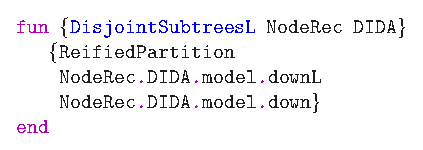
\includegraphics[scale=1.0]{eps/opti2}
\end{center}
wobei {\tt ReifiedPartition} eine reifizierte Version des Constraints
{\tt FS.partition} aus der Oz-Finite-Set-Constraints-Bibliothek
ist.

\subsection{Informelle Analyse der Optimierung}

Der Optimierer kann noch deutlich mehr Pattern erkennen als wir hier
vorgestellt haben. Die Optimierungen machen exzessiv Gebrauch der
Mengen aus den Modellen. Dabei eliminieren sie Quantifizierungen und
verringern die Anzahl der gestarteten Propagierern.

Erste Vergleiche zwischen optimierten Prinzipien, die vom
PrincipleWriter generiert wurden, und unoptimierten generierten
Prinzipien, sowie schon vorhandenen Prinzipien, die von Experten von
Hand optimiert wurden, haben gezeigt, dass die automatisch optimierten
Prinzipien deutlich effizienter sind als die unoptimierten. Die
automatisch optimierten Prinzipien sind zwar nicht ganz so schnell wie
die von Hand optimierten, sie sind allerdings jetzt schon effizient
genug f\"ur den praktischen Einsatz, gerade zum Experimentieren mit
neuen Prinzipien.

Verglichen wurden zwei Grammatiken aus der XDK-Distribution. Die
Nutshell-Einf\"uhrungs-Grammatik (nut1.ul) aus \cite{Debusmann06}, die
eine vereinfachte englische Grammatik ist mit einer
Syntax-Semantik-Schnittstelle. Sie hat drei Dimensionen, 12 Prinzipien
und ein kleines Lexikon.  Die zweite Grammatik war die gro{\ss}e
Grammatik aus der Dissertation von Ralph Debusmann, die ebenfalls eine
Englische Grammatik ist, mit 12 Dimensionen, 53 Prinzipien und einem
gro{\ss}en Lexikon.  F\"ur beide Grammatiken wurden zwei
repr\"asentative S\"atze getestet. Einmal mit den vom PrincipleWriter
optimierten Prinzipien, und einmal mit den von Hand optimierten. Die
Ergebnisse waren folgende:
\begin{center}
\begin{tabular}{| r | c | c|}
\hline
 & Nut1.ul & Diss.ul \\
\hline
Handoptimiert & 94 & 1.46 \\
 & 109 & 0.655 \\
\hline
PWUL-nicht-Optimiert &  375 & 17\\
 & 468 & 5.65\\
\hline 
PWUL-Optimiert & 172 & 10.21 \\
 & 234 & 2.57 \\
\hline
\end{tabular}
\end{center}
Diese ersten Tests haben einerseits gezeigt, dass die Prinzipien, die
durch den PrincipleWriter generiert wurden, alle Prinzipien abdecken,
die die Diss-Grammatik beinhaltet. Das ist ein guter Test, da die
Diss-Grammatik fast eine Obermenge aller bisher benutzten Prinzipien
benutzt.  Dass die Optimierungen greifen kann man anhand der
Parsezeiten sehen. Bei beiden Grammatiken sorgen sie f\"ur eine
Effizienzsteigerung von mehr als 100\%.  und kommen der Effizienz der
von Hand optimierten Prinzipien recht nahe. Bei der gro\"ssen,
aufw\"andigen diss-Grammatik sind die optimierten Prinzipien immer
noch ca.\ doppelt so schnell wie die nichtoptimierten, aber ca.\ 5mal
langsamer als die von Hand optimierten.
%diss

%opti
%10.21
%2.57

%handopti
%1.46
%0.655

%--

%nut1

%noopti
%375
%468

%opti
%172
%234

%handopti
%94
%109

Es bleibt also Spielraum f\"ur weitere Forschungen, wie die Prinzipien
noch besser automatisch optimiert werden k\"onnen. In der jetzigen
Version sind die Optimierungen aber ausreichend, um viele neue
Prinzipien aufzuschreiben, ohne sich um die Optimierung Gedanken
machen zu m\"ussen, und damit neue Ideen f\"ur dependenzbasierte
Grammatikformalismen zu explorieren.
